\documentclass{article}
\usepackage[margin=1.0in]{geometry}

\usepackage{amsmath}
\usepackage{amsfonts}
\usepackage{amssymb}
\usepackage{graphicx}
\usepackage[hidelinks]{hyperref}
\usepackage{showlabels}
\usepackage{lineno}
\linenumbers

\newcommand{\median}{\operatorname{median}}

% http://bytesizebio.net/2013/03/11/adding-supplementary-tables-and-figures-in-latex/
\newcommand{\beginsupplement}{%
        \setcounter{table}{0}
        \renewcommand{\thetable}{S\arabic{table}}%
        \setcounter{figure}{0}
        \renewcommand{\thefigure}{S\arabic{figure}}%
     }

\hyphenation{Ge-nome Ge-nomes hyper-mut-ation through-put}

\title{Phage Immuno-Precipitation Sequencing (PhIP-Seq) Pipeline to characterize antibody targets for SARS-CoV-2}
\author{Jared G. Galloway}

% QUESTION: Where should we squeeze in phage-dms explanation? discussion?

\begin{document}
\maketitle

\begin{abstract}
The adaptive immune system interacts and identifies pathogens in the body by identifying a "molecular key" unique to that pathogen.
When an individual is exposed to the pathogen, a full adaptive immune responce can generate a surpluss of antobodies which can bind specifically to that key.
Identifying this molecular key for pathogens of interest remains an outstanding problem crutial to designing vaccines. 
Phage Immuno-Precipitation Sequencing (PhIP-Seq) is a powerful protocol for investigating potential antibody targets (epitopes) \cite{Larman2011}. 
Concretely, this workd by investigating protein-protein interactions between the human body's own antibodies with artificial epitopes displayed on phages (phage vectors).
The key assumption being that recovered patients who have undergone 
a full adaptive response to a disease we care about will have high enough volumes of antibodies (IgG content) to accurately observe an interaction with the pathogen causing the disease. 
Here, we provide and explore two related computational tools created for this data;
(1) An analysis pipeline that takes in demultiplexed next generation sequencing files and produces a coherent dataset to explore the data.
(2) A python package, dubbed \textbf{phippery}, to query this dataset.
Finally, we demostrate the use of this pipeline by applying it to SARS-CoV-2 dataset.
\end{abstract}

\section*{Introduction}

The immune system is most simply divided into two biological mechanisms which we call the innate and adaptive immune systems.
The innate immune system primarily made of cells, such as leukocytes, which can primarily clasify an object as either foreign or native to the body.
this allows for the body to repond quickly to pathogens and invokes reponses that are non-specific to the pathogen it is responding to.
If the pathogen survices these initial attackis, the body's second wave of defence is a more specifc attack known as the adaptice immune responce.
The adaptive immune responce relies upon generating antibodies which can identify a singular pathogen which induced the response. 
Antobodies are used primarily to tag a pathogen which will can then signal a specialized cell, such as a natural killer cell (NKC) to destroy the pathogen. 
Perhaps the most amazing part of the adaptive immune system is it's ``memory" for a pathogen it has encountered in the lifetime of the host organism.
 
When designing vaccines for viruses, the memory of the adaptive immune system is leveraged by provoking the immune respose with a nuetralized representation of a certain virus.
This provides the host organism with the right set of cells to respond to the real virus when it is encountered. 
Perhaps the largest obsticle when designing vaccines is the genration of a neutral pathogen that accurately embodies the features of the real virus.
To do this, it is often necessary to understand the molecular key -- a peptide chain -- which antibodies use to bind to the pathogen and tag it for later destruction.
Identifying this protein, often referred to as the epitope, remains a large challenge in the field. 
Knowing that the oligonucleotide sequence encoding for this protein lives somewhere where in the genome of the pathogen,
researchers can leverage Next Generation Sequencing (NGS) and Synthetic Oligonucleotide Generation (SONG)
to display a large range of possible epitopes on the surface of a phage.
Those phages are then exposed to antibodies from recovered patients and protein interactions are explored using novel technique known as 
Phage Immuno-Precipitation Sequencing (PhIP-Seq) \cite{Larman2011}.

PhIP-Seq works by synthesizing an array of proteins -- each of which could potentially model the epitope of pathogen -- 
then cloning the repspective genetic "tiles" (oligonucleotides encoding peptides) into a phage vector of choice. 
Samples from a patient's serum antibodies are mixed with magnetic beads and phages to capture the enrichment of phages-antibody interaction.
After an immunoprecipitation, the phages-inserted oligos caught on the magnetic beads are prepped for sequencing, amplified, and barcoded. 
Using Next generation sequencing, 
researchers can then quantify the number of each unique oligos representing a peptide captured in the immunoprecipitation step using short read alignment. 
The analysis of these datas consists demultiplexing the samples,
then aligning the peptides to the reference library in order to generate a count of each specific peptide and sample combination. 
The final result is in the form of a matrix, $X$, where (heuristically) there is a row, $i$, for each peptide and a column, $j$, for each sample.
Concretely, $X_{j,i} =$ the number of reads from sample $i$, which contain the peptide $j$.

Doing analysis for this protocal presents two challenges:
(1) This protocal requires an immense amount of book-keeping and computational power to produce coherent results.
(2) From this protocol, there are a variety of sources from which one can expect add noise to the resulting data, t
hese are including but not limited to; 
IgG content of a sample, "immuno-dominant" antibodies, sequencing bias (GC-content?), amplification bias, and phage display (total amount of each phage in the phage library). 
Here, we describe a pipeline we constructed to handle all bookkeeping and can run the alignment and counts merging steps in parallel to produce a coherent counts matrix with metadata for each sample and peptide.
Additionally, we provide some preliminary results analyzing this data using a python package, \textbf{phippery}, specifically designed for the output of the pipeline.

\section*{Methods}

1. a more in-depth explanation of the pipeline. possibly outlining the advantages and portability of nextflow.

The nature of sample alignments to the peptide encoding oligo sequence reference library makes this a perfect candidate for a workflow manager which 
can perform these steps in parallel on a high performance computer (HPC). 
For this specific pipeline we use Nextflow paired specialized docker containers to produce a reproducible and highly-parallized workflow \cite{Merkel_2017, DiTommaso2017}.
Figure \ref{fig:DAG} shows the directed acylclic graph (DAG) of the pipeline from input metadata and sequencing file to a specialized python object containing
the repective counts and metadata for each sample and peptide \cite{van1995python}.

\begin{figure}[h!!!!]
\centering
    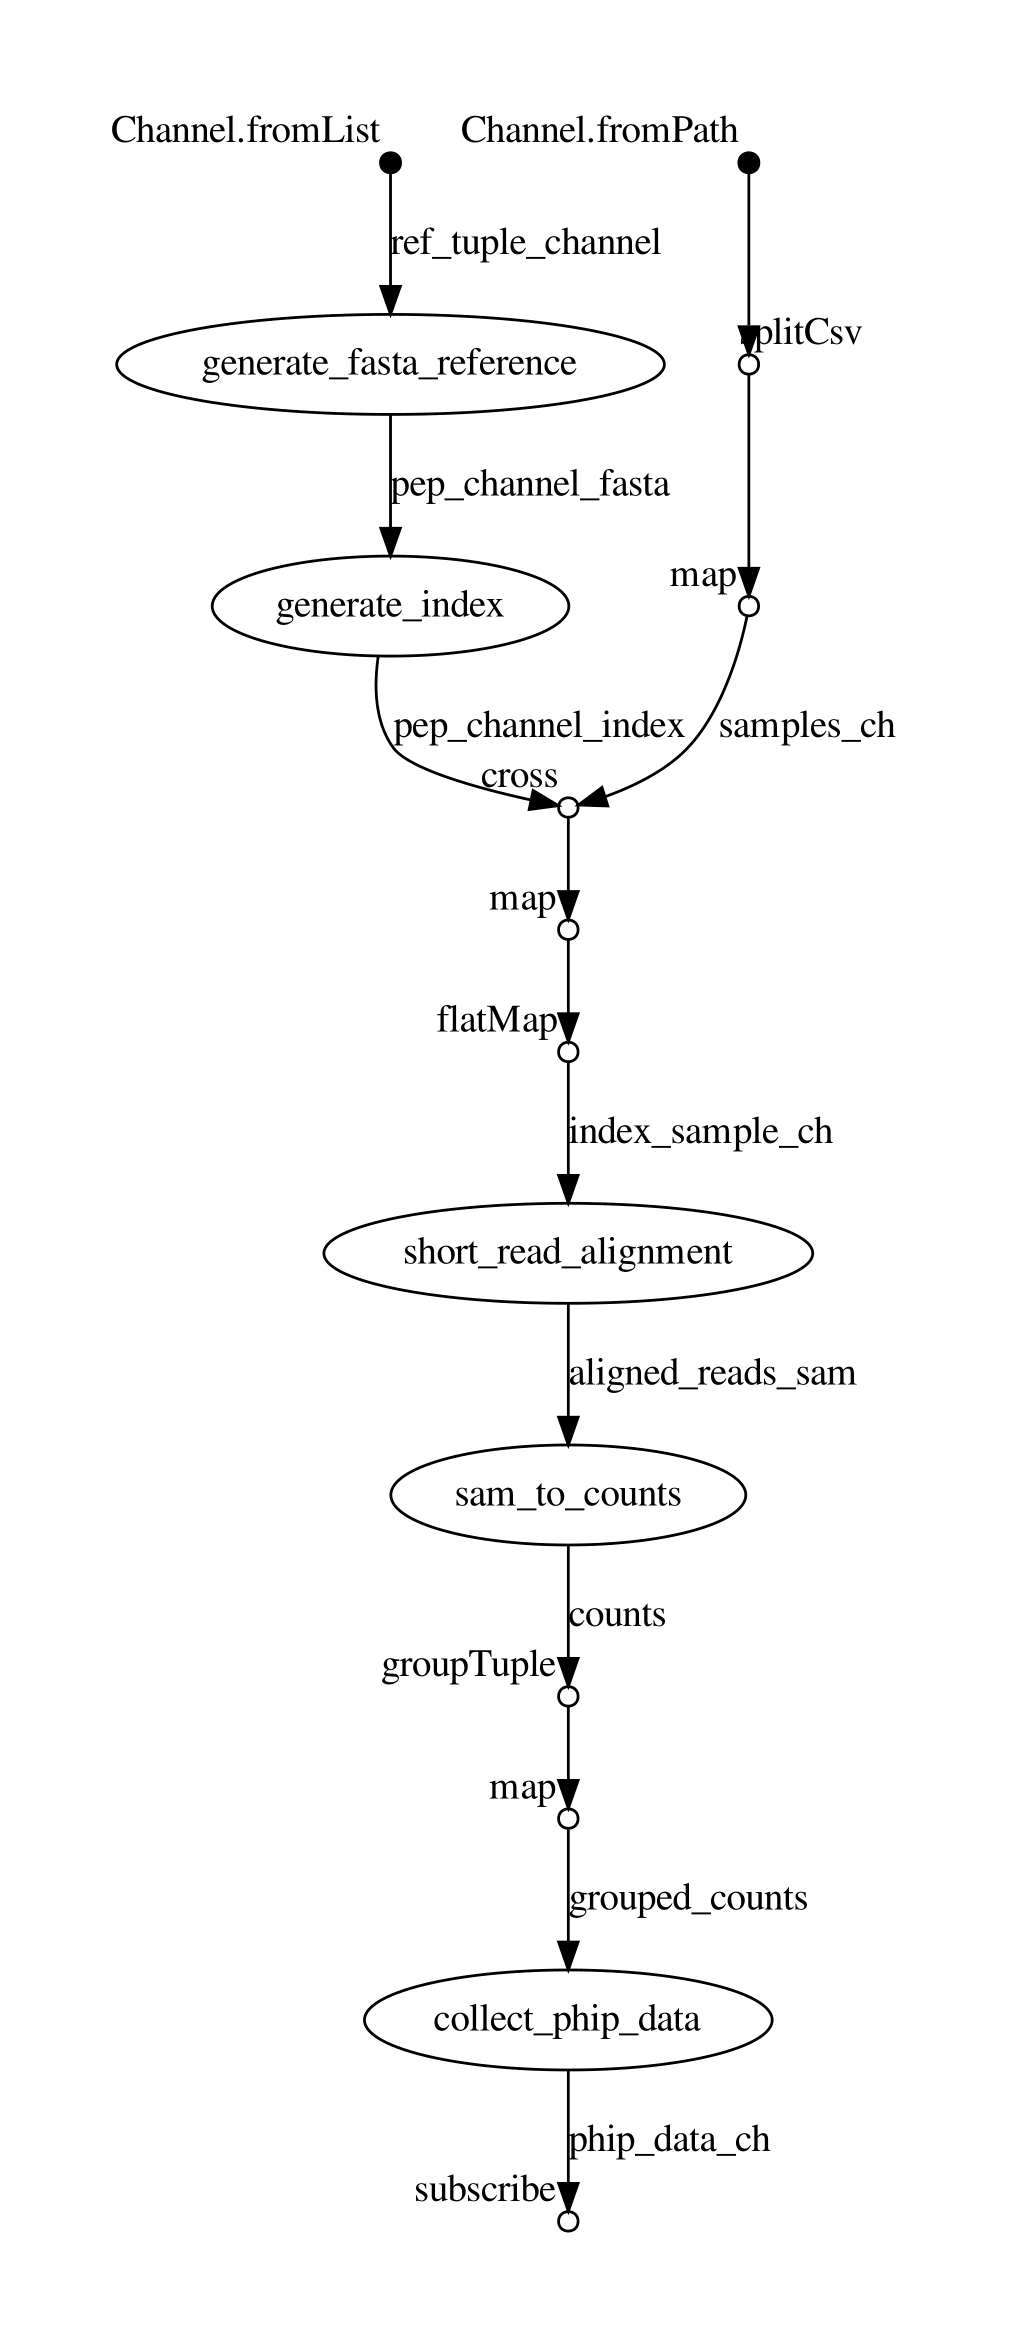
\includegraphics[width=0.35\textwidth]{figures/dag-1.png}
    \caption{DAG.}
\label{fig:DAG}
\end{figure}

3. a brief explanation of tools used at each step of the pipeline

% \begin{figure}[h]
% \centering
% \includegraphics[width=0.35\textwidth]{figures/subsplit.pdf}
% \caption{\
% A subsplit structure.
% }
% \label{fig:subsplit}
% \end{figure}

\subsection*{Pipeline Input - Data}

$\approx 2 - 3 pages$

\paragraph{Sample metadata}
\paragraph{Peptide metadata}
\paragraph{config file}

\subsection*{Pipeline Output}

1. Describe the counts generated

2. A figure showing the heatmap of counts.

 \begin{figure}[h!!!!]
 \centering
 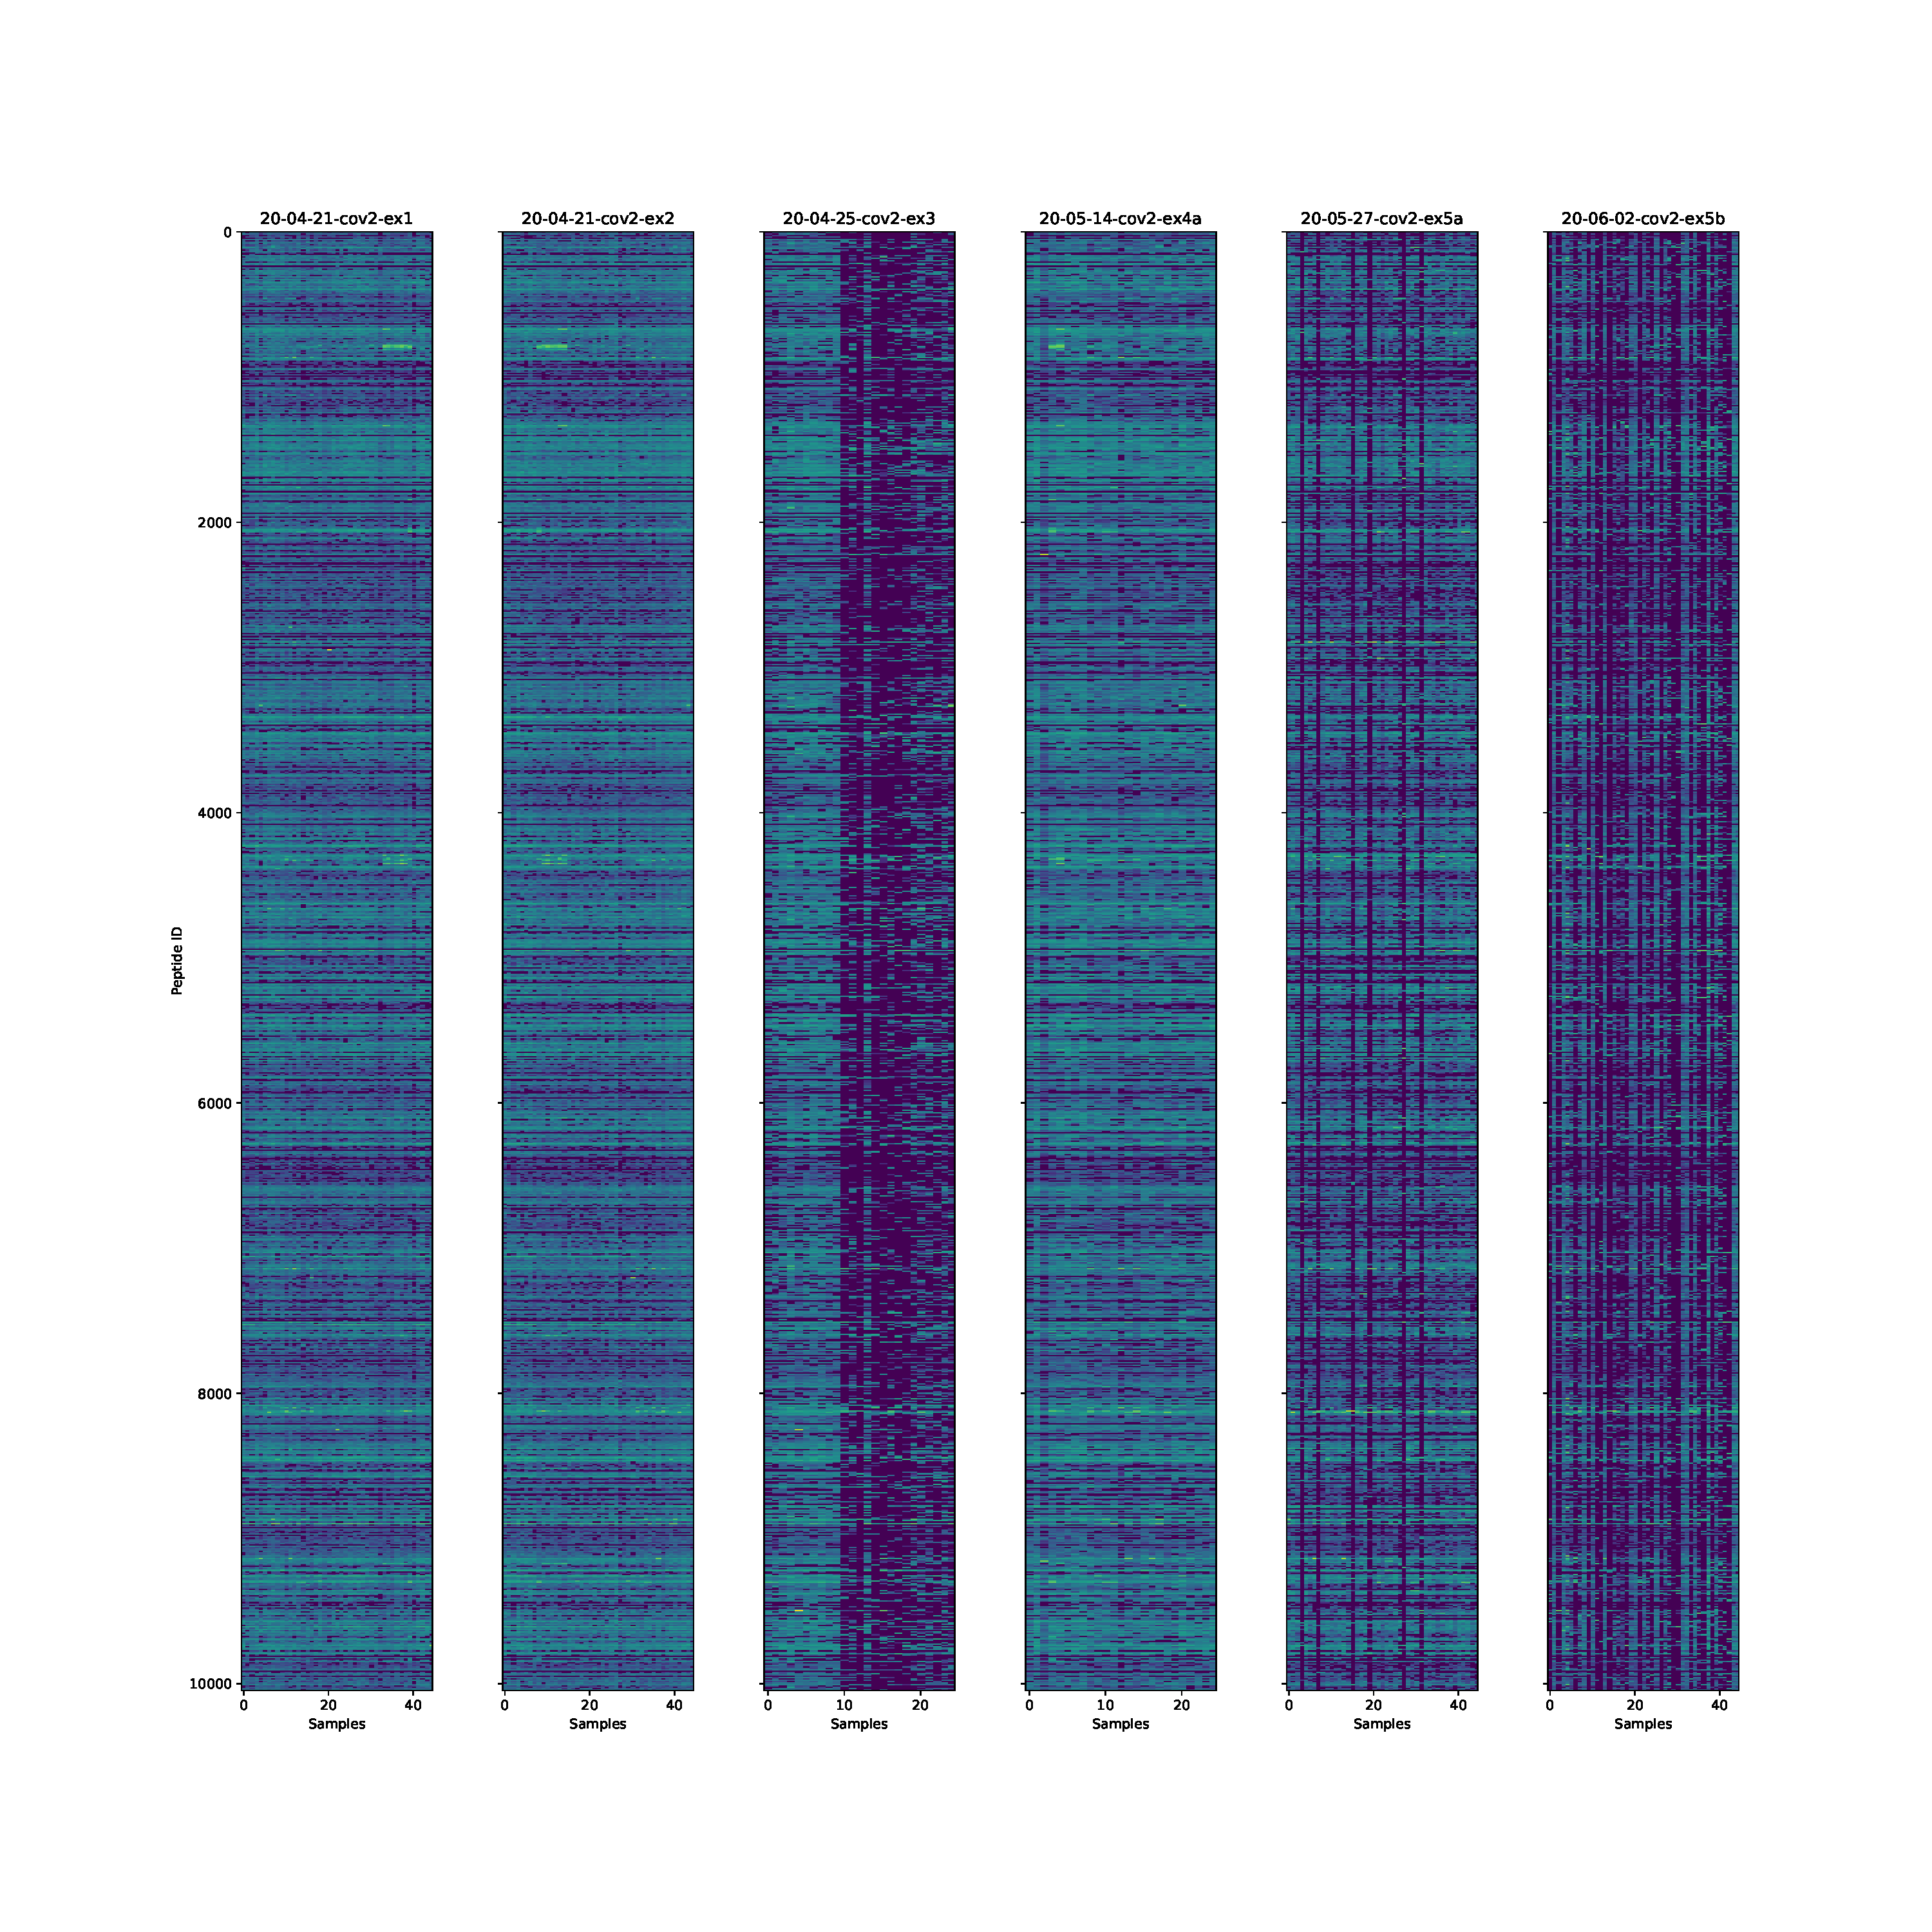
\includegraphics[width=1.0\textwidth]{figures/raw_counts.pdf}
 \caption{ \
 Raw counts.
 }
 \label{fig:raw_counts}
 \end{figure}

\section*{Results}

$\approx 1 page$

1. Introduce phippery and 

\begin{figure}[h!!!!]
\centering
\includegraphics[width=1.0\textwidth]{figures/correlation_by_experiment_sample_type.pdf}
\caption{ \
Technical Replicates
}
\label{fig:tech_reps}
\end{figure}

\begin{figure}[h!!!!]
\centering
    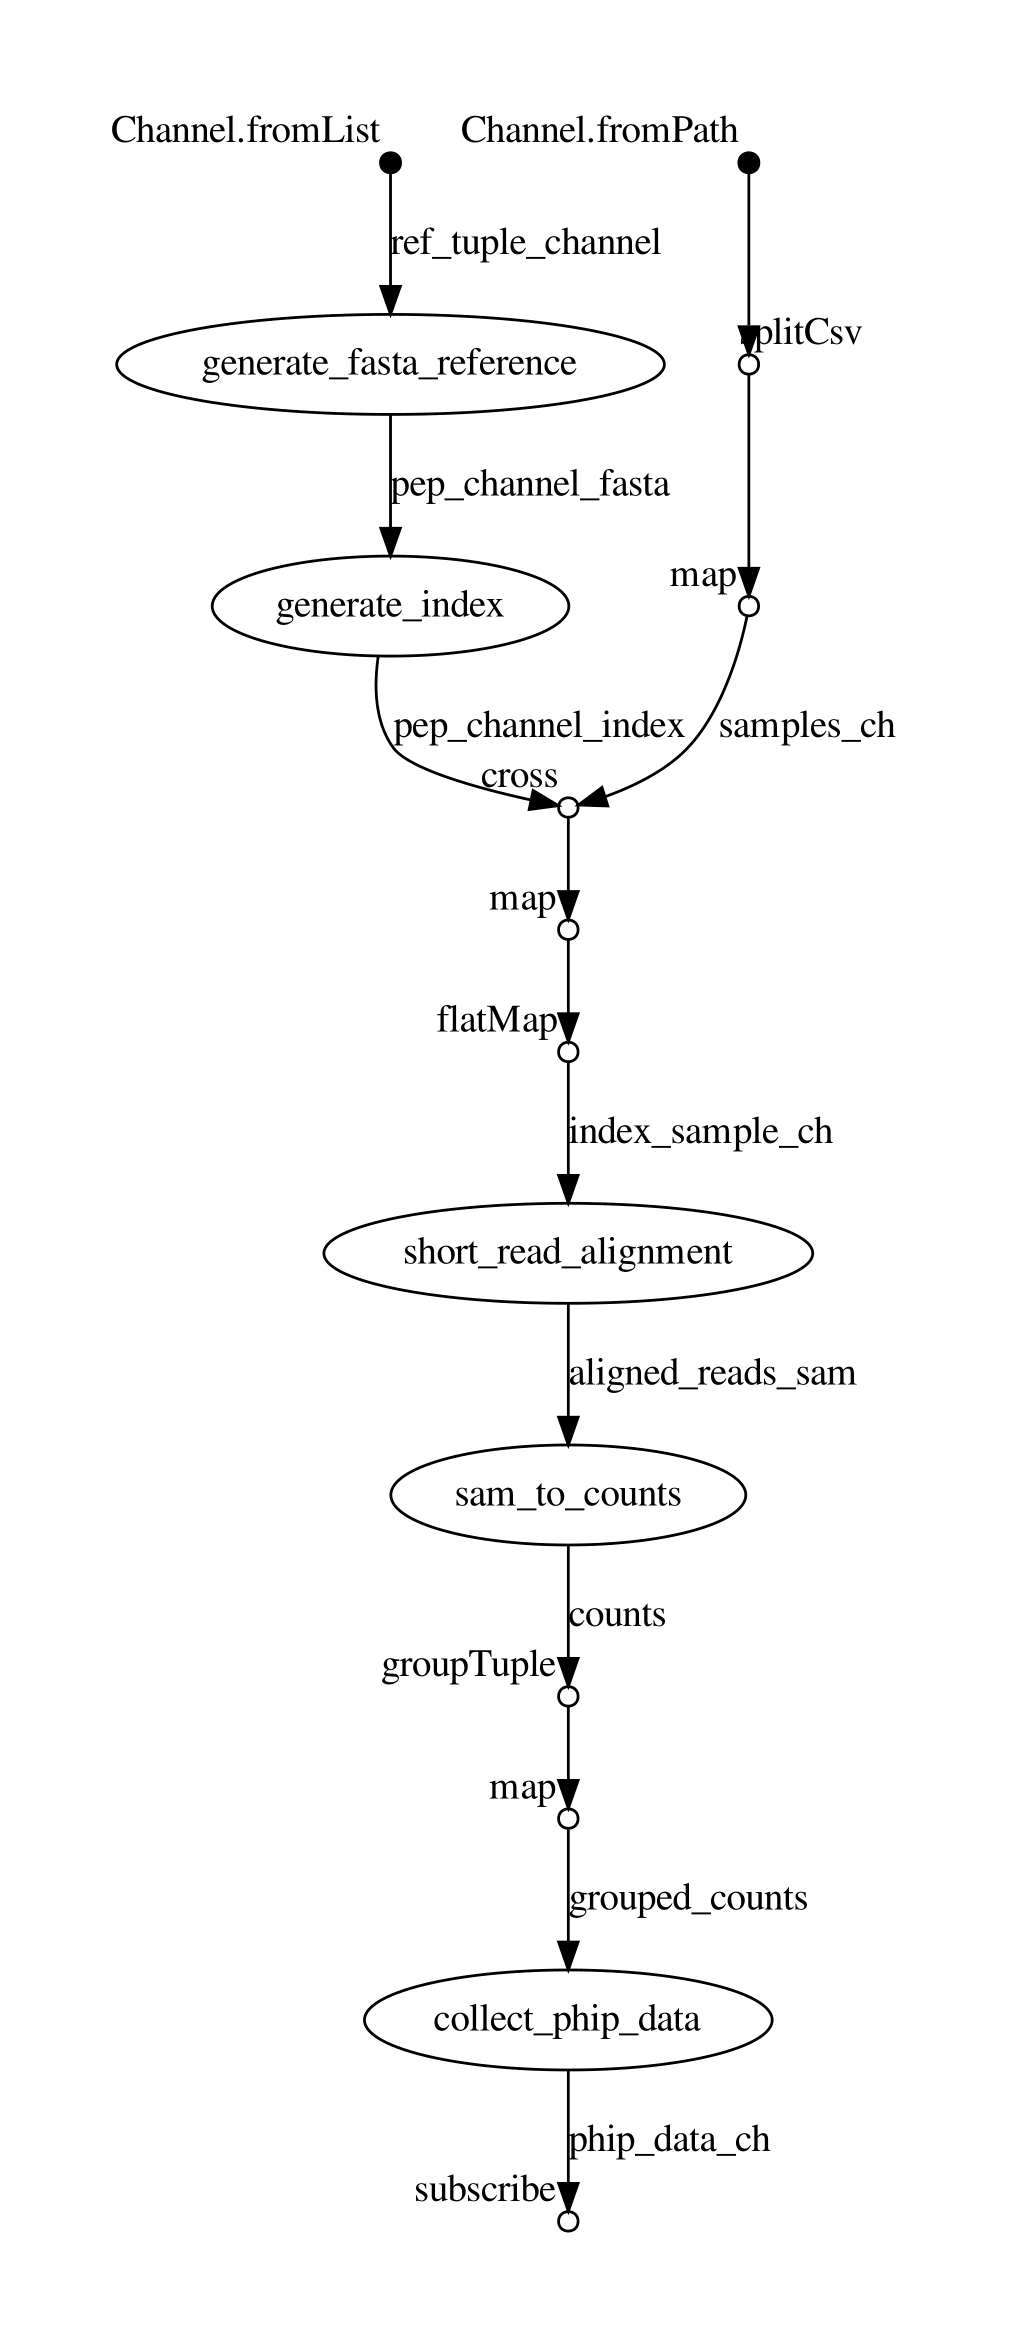
\includegraphics[width=0.35\textwidth]{figures/dag-1.png}
    \caption{DAG.}
\label{fig:DAG}
\end{figure}

Figure \ref{fig:tech_reps}

2. general approach to query data of this type.

3. Some fold enrichment plots?

% \begin{figure}[h]
% \centering
% \includegraphics[width=0.35\textwidth]{figures/subsplit.pdf}
% \caption{\
% A subsplit structure.
% }
% \label{fig:subsplit}
% \end{figure}

\paragraph{Fold enrichment}

4. Describe fold enrichment and what our results tell us so far.

\section*{Discussion \& literature review}

$\approx 1-2 pages$

Good place to review some recently used methods moving forward, and concerns we have?

\paragraph{z-score}

\paragraph{motif analysis}

...


\bibliographystyle{plain}
\bibliography{main}

% \clearpage
% \section*{Supplementary Materials}
% \beginsupplement
% Supplementary text and figures here.


\end{document}




